\section{Local and short-term variability of the detached haze layer}

So far, we have considered the evolution of the detached haze layer in the frame of the seasonal change.
We then discussed the long term-evolution at the planetary scale as a function of latitude.
In this section we consider sets of observations to characterize local and short-term
behavior of the detached haze. First, we choose several images taken a few hours apart to
evaluate the hourly variability of the detached haze. Next, we consider
observations at low phase angle which show simultaneously the two limbs of Titan. And, finally,
we consider observations taken from a near-polar point of view which can show
longitudinal variations in a narrow range of latitudes.

\subsection{Short time or spatial  variability}

As presented before, we observe between December 2004 and June 2005 a large amplitude variability of the
detached haze layer extinction profile at all the latitudes below \ang{35}N (Fig.~\ref{fig:dhl_2004_2008}a
to \ref{fig:dhl_2004_2008}c). Fortunately, Cassini took in June 2005 a series of 9 images of
Titan with a time-step of 80 minutes apart (Table.~\ref{tab:time_variability}).

\begin{table}[!ht]
    \centering
    \caption{Sequence of the 9 images of Titan taken June 4$^{th}$, 2005.
    The longitude and local time are given for the profile at the equator
    on the illuminated side of Titan.}
    \vspace{.5cm}
    \begin{tabular} {c c c c c}
        \toprule
        Imag ID & Time (UTC) & Phase & Longitude (Eq) & Local Time (Eq)\\
        \midrule
        N1496548825\_1 & 03:32 & \ang{10.4} & \ang{10.7}W & 17:12 \\
        N1496552665\_1 & 04:36 & \ang{10.3} & \ang{10.4}W & 17:17 \\
        N1496557465\_1 & 05:56 & \ang{10.1} & \ang{10.6}W & 17:23 \\
        N1496562265\_1 & 07:16 &  \ang{9.9} & \ang{13.1}W & 17:17 \\
        N1496567065\_1 & 08:36 &  \ang{9.8} & \ang{13.4}W & 17:23 \\
        N1496571865\_1 & 09:56 &  \ang{9.8} & \ang{13.9}W & 17:23 \\
        N1496576665\_1 & 11:16 &  \ang{9.8} & \ang{14.3}W & 17:30 \\
        N1496581465\_1 & 12:36 &  \ang{9.9} & \ang{14.7}W & 17:30 \\
        N1496586265\_1 & 13:56 & \ang{10.1} & \ang{15.2}W & 17:36 \\
        \bottomrule
        \label{tab:time_variability}
    \end{tabular}
\end{table}

With multiple observations of Titan in a short period, we are able to validate our calibration and
observe short time and local variabilities. Here, we analyze the sequence at three different
locations on the limb (\ang{40}S, \ang{0}, \ang{40}N). The 9 observations are made with phase
angles around \ang{10}, within an interval of \ang{0.6}. The limb longitude of the observations
varies  between \ang{10}W and \ang{15}W whereas the solar local time on Titan varies between
17:12 and 17:36.

\begin{figure}[!ht]
    \centering
    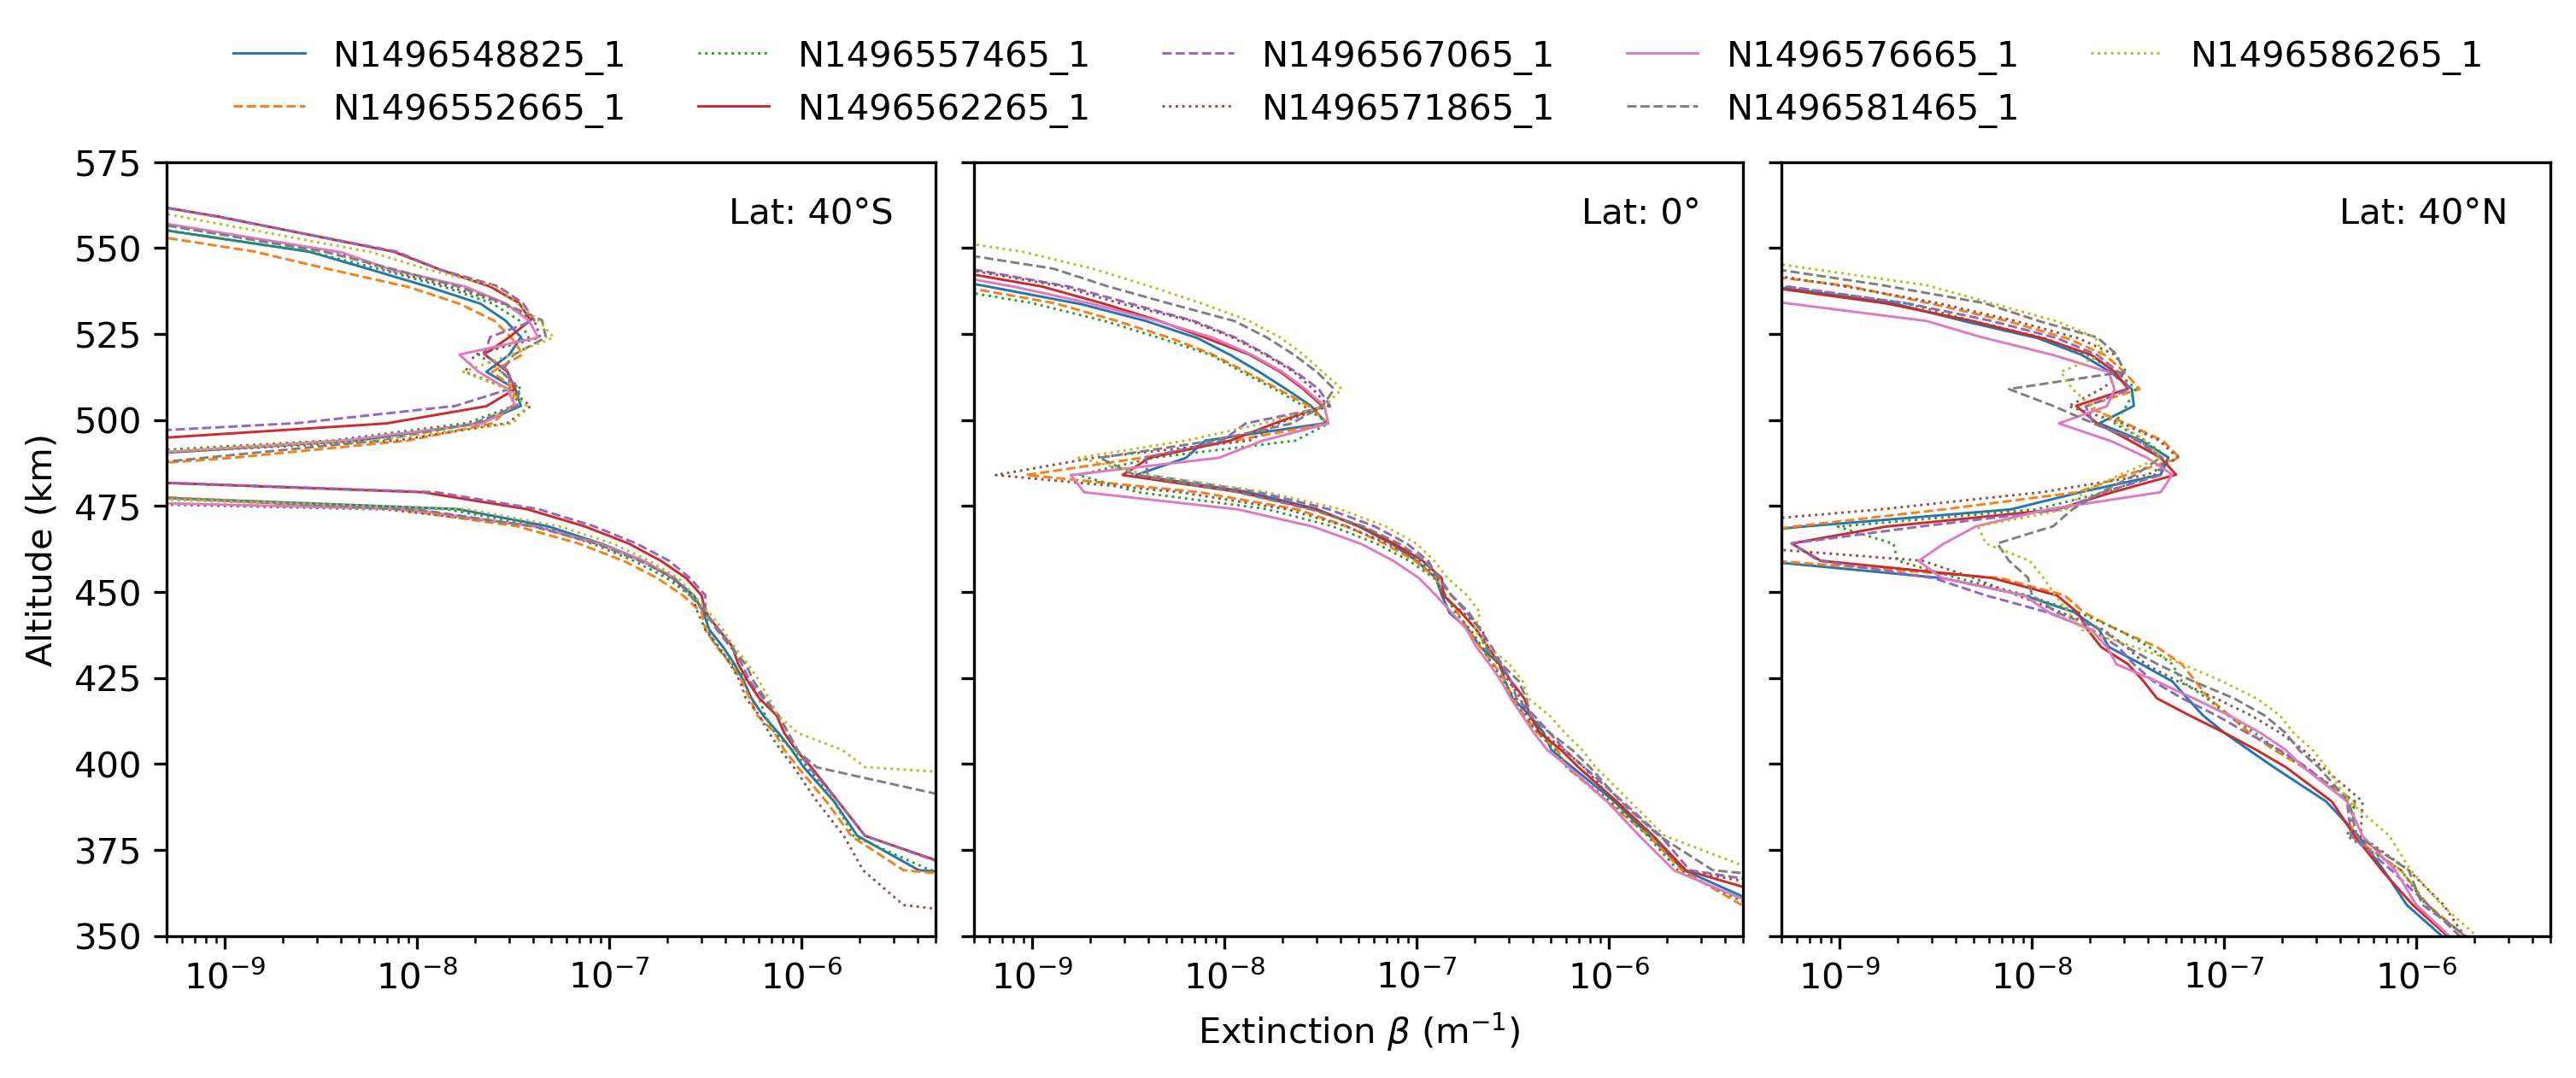
\includegraphics[width=\textwidth]{Fig/Time_variability.png}
    \caption{Extinction profiles for the series
    of 9 images taken 80 minutes apart in June 2005 (cf. Table \ref{tab:time_variability}).
    The global latitudinal map is shown in figure~\ref{fig:dhl_2004_2008}c.}
    \label{fig:time_variability}
\end{figure}

The figure~\ref{fig:time_variability} presents extinction profiles extracted from the analysis of these 9 images.
First, we confirm that our calibration method is reliable from one picture to the other and the overall
variability of the detached haze is very small. We clearly observe the double layering at \ang{40}S and \ang{40}N reported
previously. All the locations of the maximum of the extinction peaks are located within a small altitude range (smaller
than the 8 km of the pixel scale). Then, the vertical offsets which are observed at different times are consistent
with  the accuracy of the image navigation, and therefore are not significant. At the equator and at \ang{40}S, the detached
haze layer is well detached for all the profiles. When the vertical offset is accounter for, all the extinctions are found
with relative differences of about $\pm$ 10\% compared to the average value, except in the depletion zone between
the main and detached haze layers where difference can reach an order of magnitude (at \ang{0}) to several order of magnitude
(\ang{40}N). The variations outside the depletion zone are not significant. We note that the different behavior of the
N1496576665\_1 profile at \ang{40}S and below 450 km, compared to other profiles, is an artefact due to the inversion
process.

The variability in the depletion zone at the equator is probably due to the retrieval uncertainties. The differences in
extinction are about one order of magnitude, consistent with uncertainties between the two layers
\citep[\emph{e.g.}][]{West2018}, and without specific temporal evolution.
The variability observed at \ang{40}N, in the depletion zone around 460 km are significant for two reasons.
First, the differences are much larger than the expected uncertainty in this zone. Second, the sequence shows
a gradual and consistent increase of extinction with time. If these differences were due to uncertainties in
the retrieval procedure, it would have rather given a chaotic evolution of the extinction with time.

We also remark that the corresponding extinction map (Fig.~\ref{fig:dhl_2004_2008}c) shows that in the south,
the detached haze is well separated from the main haze by a well defined depletion zone. In the north, the depletion
zone is less well defined and the detached haze and the main haze are connected vertically by a residual haze.
The variation of this residual haze is the one reported in Fig.~\ref{fig:time_variability} at \ang{40}N.
We can not strictly determine if we are witnessing time or a spatial variations since both the time and the longitude
of the observations change simultaneously during the image sequence. We note that a rotation of \ang{5} in longitude
corresponds to a maximum shift of 250 km in distance (one tenth of Titan radius), possibly consistent with a spatial
variation of the haze extinction.

\subsection{Dawn and dusk sides}

Aside from short time and local variations, we also are interested in images showing simultaneously the two sides
of Titan. At low phase angle, the viewing geometry allows us to retrieve the haze extinction with both the
illuminated and the dark side of Titan simultaneously  (Fig.~\ref{fig:dawn_dusk}).
In this case, we can compare the dawn and dusk limbs for
specific latitudes. Although Titan's day is about 16 terrestrial
days, the time spent by the haze on the night side or dayside is much shorter.
First, the atmosphere is superrotating and at altitude around 400 or 500 km the zonal wind is comparable to or
larger than the rotation speed at the ground \citep{Flasar2005, Achterberg2011, Lebonnois2012, Lellouch2019}.
This makes the actual diurnal cycle for the high altitude hazes shorter than 16 days by a factor of 2 or more.
Secondly, at high altitude, sunlight penetrating beyond the geometric terminator further shortens the time spent in darkness.
Thus, effects on the haze should be produced by processes with timescales
comparable with a terrestrial day.

\begin{figure}[!ht]
    \centering
    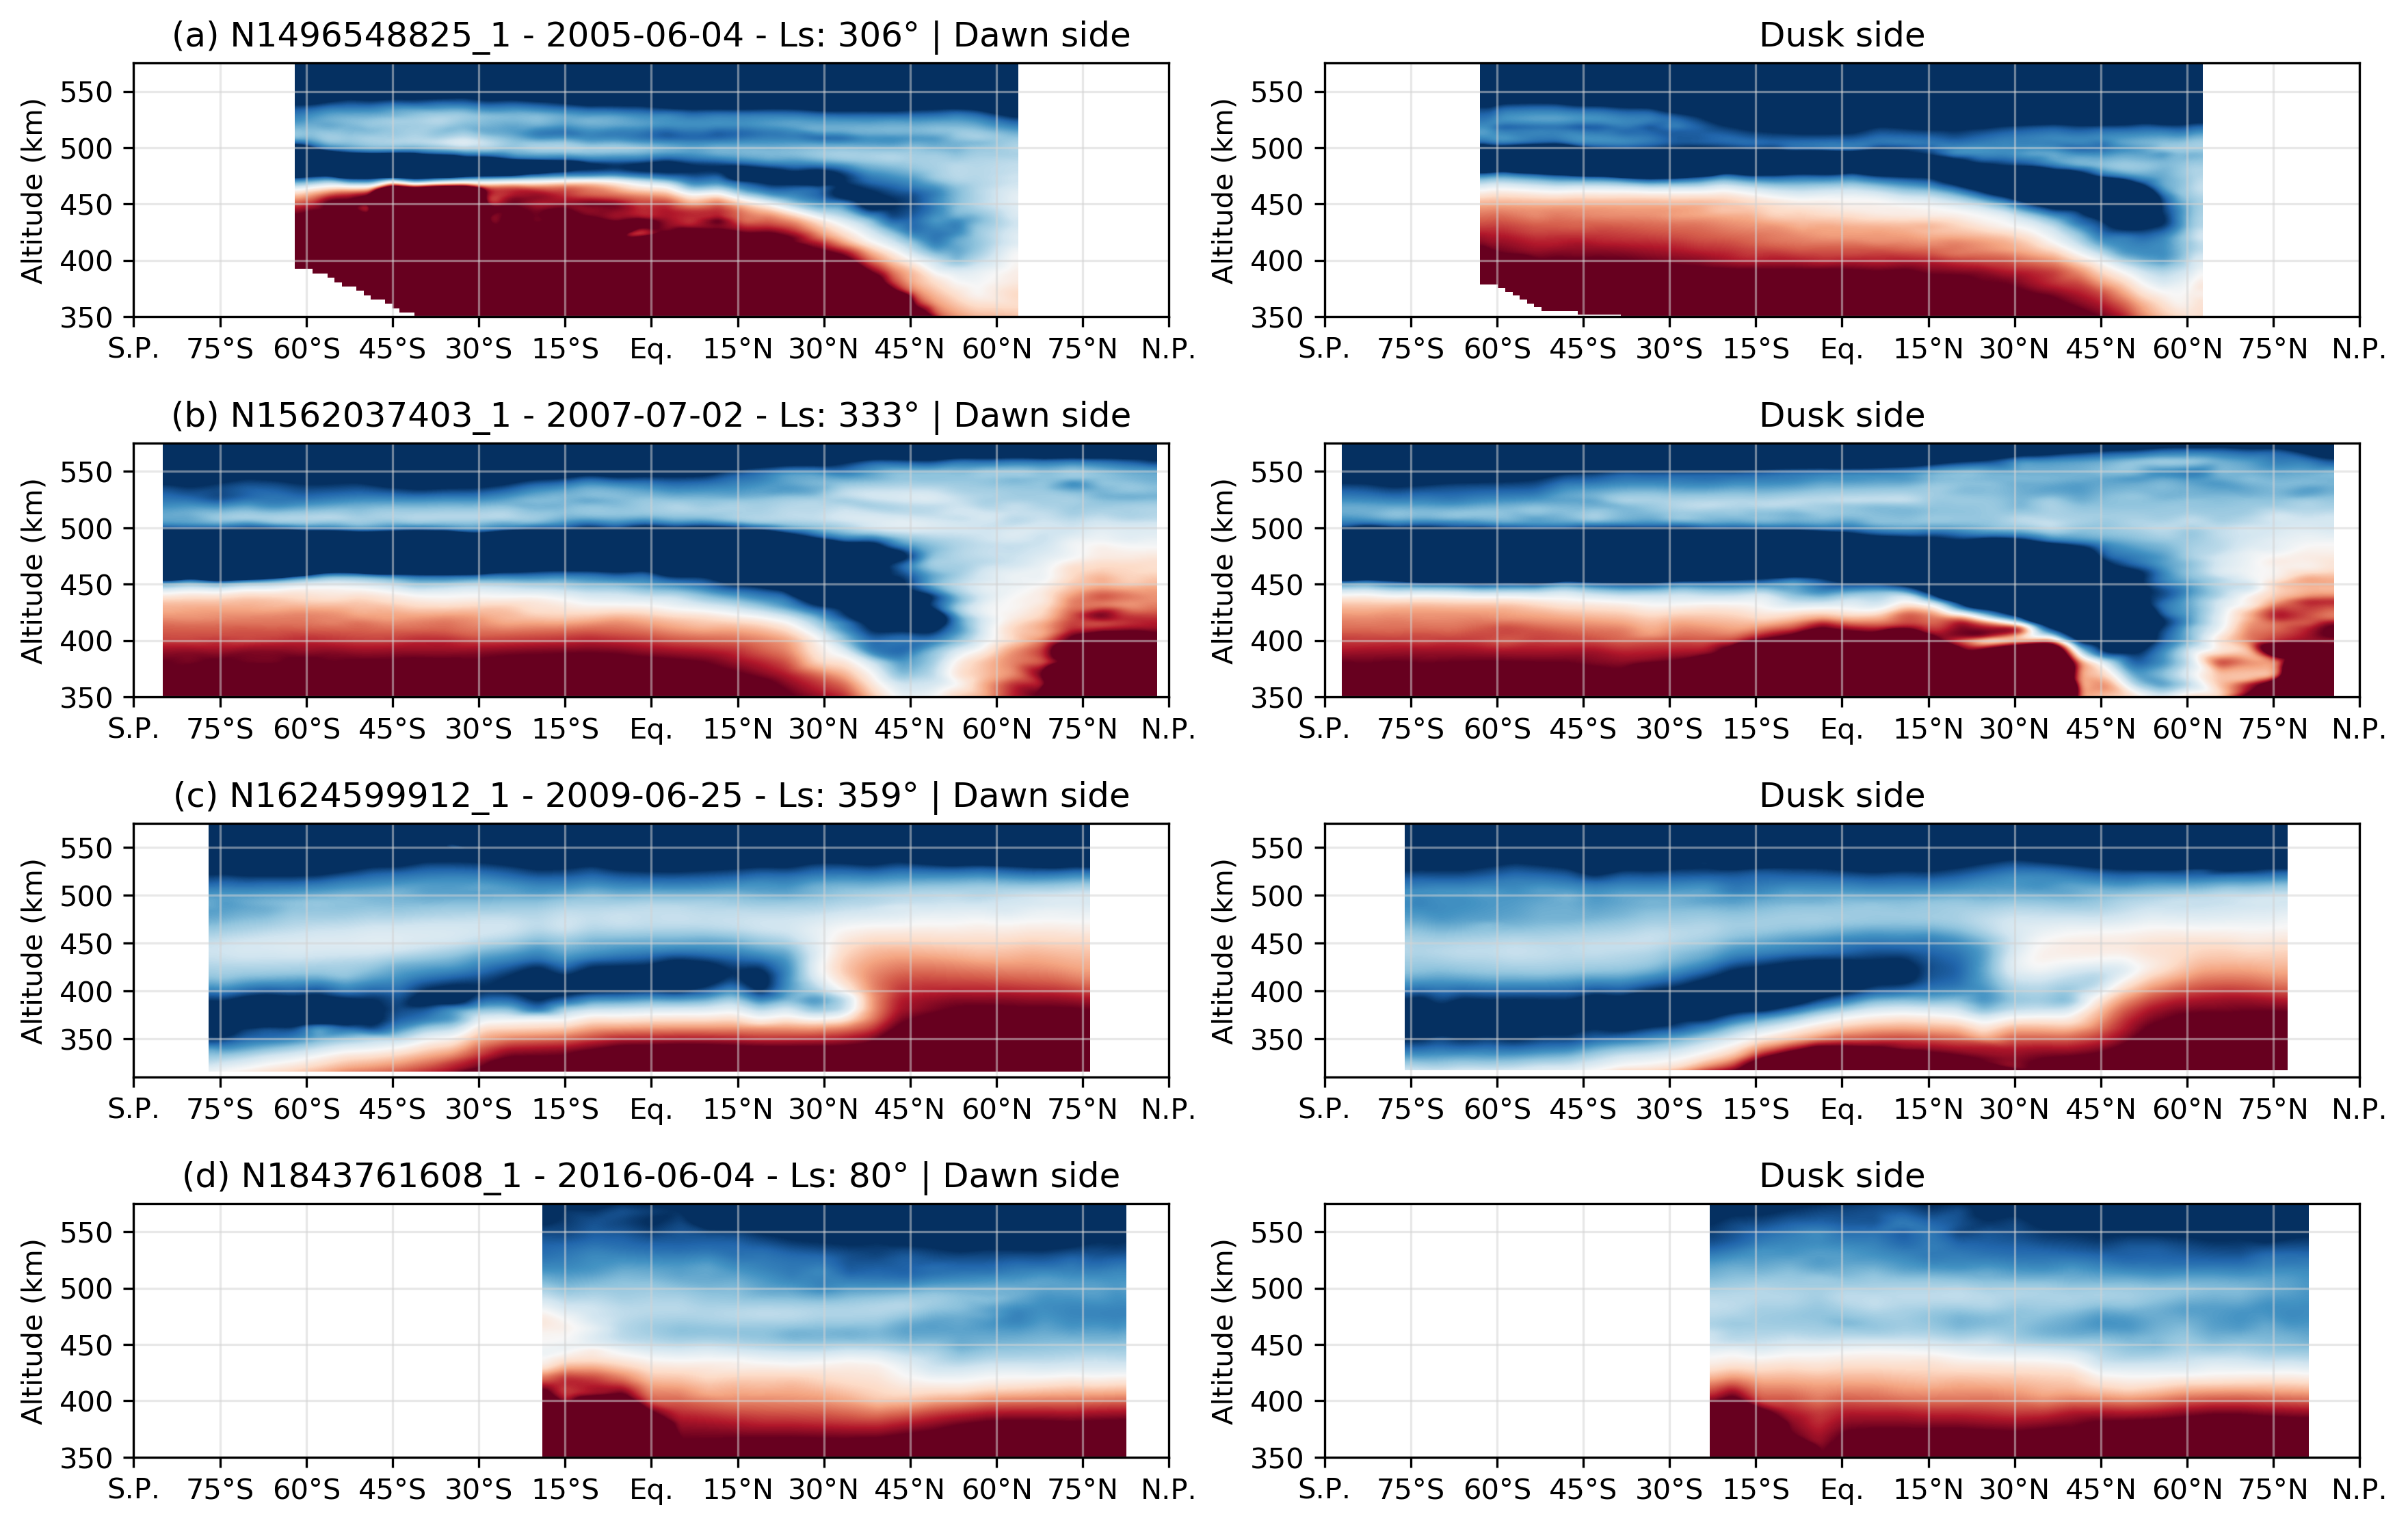
\includegraphics[width=\textwidth]{Fig/Dawn_dusk.png}
    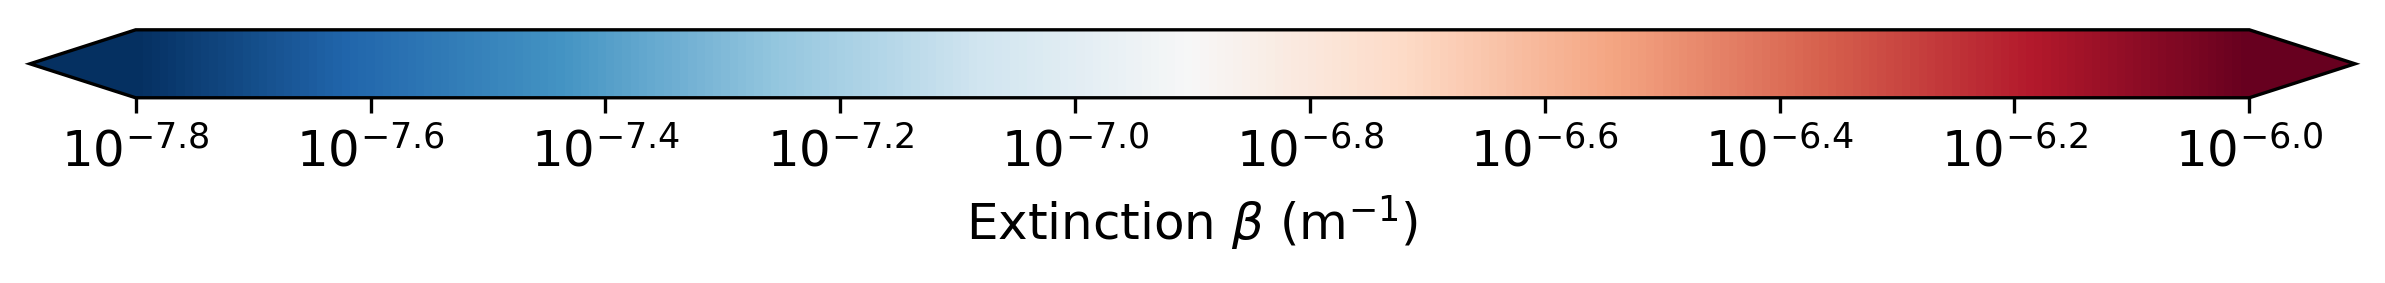
\includegraphics[width=.5\textwidth]{Fig/Extinction_colorbar.png}\vspace{-.3cm}
    \caption{The left and right panels show maps of the haze extinction for the dawn and dusk side of
    Titan for 4 different images taken during the mission when the viewing geometry allows us to observe both dawn and dusk
    limbs. The date and the seasonal solar longitude are provided for each image.}
    \label{fig:dawn_dusk}
\end{figure}

Figure~\ref{fig:dawn_dusk}a presents the haze extinction at the dawn and dusk sides as observed
in June of 2005 (Fig.~\ref{fig:dhl_2004_2008}c). The detached haze differs significantly between the two sides.
At the equator, we observe on the dawn side a double detached layer of 40 km thickness whereas it appears
as a thin layer of 10 km thickness on the dusk side. The haze extinction at the peak differs significantly,
from 7$\times 10^{-8}$ to 2.5$\times 10^{-8}$ m$^{-1}$, respectively. The depletion below the haze layer
is also less pronounced on the dawn side compared to the dusk side. Although this observation was taken
during the period of stability for the detached haze, we observed a significant asymmetry between
the dawn and dusk side. This asymmetry is also observed in all the images taken at the same moment which were
analyzed in section 4.1.

Two years later, another low phase angle image was recorded (Fig.~\ref{fig:dawn_dusk}b).
This time, the detached haze layer is much more symmetrical between the two sides. The peaks of haze extinction
are at the same altitude with comparable values. However, small differences can be noticed: there is a
small secondary layer above the detached haze layer at the dusk side between \ang{50}S and \ang{20}N, and may even extend 
northward. In the northern hemisphere, the extinction appears slightly larger at dawn that at dusk, and the
vertical extent of the detached haze is also a bit larger. However, the overall morphologies are very similar.

At the equinox, the detached haze layer already started its drop in altitude (Fig.~\ref{fig:dawn_dusk}c).
There are significant differences between the two sides, in both hemispheres, while at the equator the two
profiles are almost identical. The haze layer is not exactly symmetrical in the southern hemisphere. The detached
haze itself is at the same altitude, but the depletion zone is at higher altitude at the dawn side, and the main
haze layer is thinner in the dusk side. In the northern hemisphere, the haze layer is more complex, and the
asymmetry is even more marked with a detached haze at different altitudes and with a different extinction. The
detached and main haze layers at the dawn side appear optically thicker than the layers at the dusk side.
This is consistent with the two previous cases.

After the equinox, fewer images were taken at low phase angle. Among them, we do not notice any
significant differences between the dawn and dusk sides. After the reappearance of the detached haze layer in
2016, we found only one image with the relevant geometry to see both sides of Titan illuminated at the same time
(Fig.~\ref{fig:dawn_dusk}d). In this case, we are close to the solstice and the sub-solar latitude is almost
at its maximal extent and does not allow us to probe the southern high latitudes near the terminator.
The main haze appears very symmetrical on both sides and almost identical
above \ang{45}N. The depletion can be followed continuously all around the North Pole. At latitudes lower than
\ang{45}N, the values of the haze extinction are similar but the altitudes of the extinction peak differ by
25 km. We also observe partial secondary detached layers in each side, but not at the same latitudes.

The haze extinction profile and the altitude of the detached haze layer can differ significantly between the dawn
and dusk sides. In general we notice a higher extinction in the dawn side than on the dusk side. This effect
could be due to a diurnal cycle.
\subsection{Longitudinal variability}

\change{Due to orbital constrains, most of our observations sampled only a small range of longitudes.
However, a few} observations of Titan taken from a near-polar point of view offer a unique way to study the evolution of
the detached haze with a large coverage in longitude and within a small range of latitudes. It allows us
first to check the homogeneity of the haze in longitude, and it also allows us to extend our previous
observations between the dawn/dusk sides with a local time coverage between 6:00 and 18:00.

\begin{figure}[!ht]
\plotone{Fig/Lon_variability}
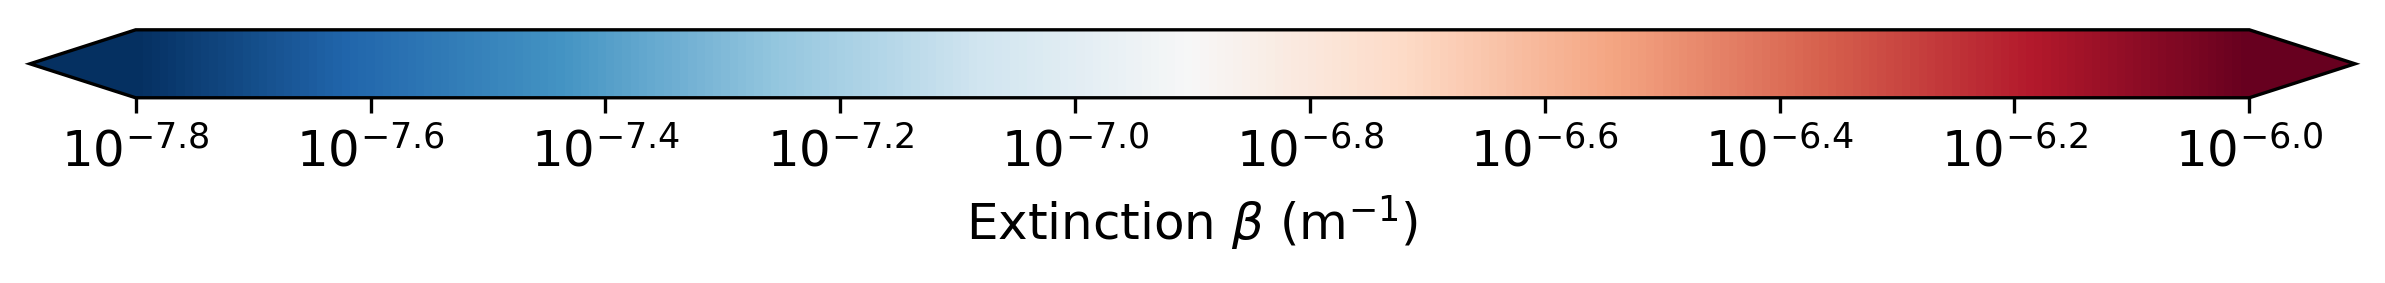
\includegraphics[width=.5\textwidth]{Fig/Extinction_colorbar}
\caption{The panels show the map of the haze extinction as a function of longitude and local
time for a set of 3 images taken in March and April, 2009 ($L_s=\ang{356}$). The latitude range covered is
also indicated for each image.}
\label{fig:lon_variability}
\end{figure}

We analyzed a set of three images taken sequentially within a month interval. The first observation
was performed on the 29$^{th}$ of March, 2009 (Fig.~\ref{fig:lon_variability}a) during the collapse of the detached
haze layer. Two other observations were made two weeks and one month later, with the same geometry
(Figs.~\ref{fig:lon_variability}b, \ref{fig:lon_variability}c). The detached haze layer is
located at 470 km at all the longitudes. Inside the depletion region, we notice a plume of haze
between 400 and 440 km and between \ang{150}W and \ang{220}W. In mid-April, the plume is located between
\ang{160}W and \ang{240}W and between 375 and 425 km. It appears disconnected and settling from the detached
layer, which remains at 470 km. At the end of April, we see the extension around 410 km and it
is spread from \ang{180}W and \ang{250}W. This aerosol plume is almost connected with the main haze.

This feature is not correlated with the local time but remains about at the same longitude and drifts slowly
toward the West. This would correspond to a retrograde motion of about 0.6 m/s. Another solution would be
prograde motion of 6.6 m/s, in phase with the sampling of 15 terrestrial days. The vertical speed, assuming
that the aerosol cloud dropped from 400 km to 375 km in one month would be $10^{-3}$ m/s. We also identified a
modulation in the extinction and in the geometrical thickness of both the detached haze layer and the main
haze. In the last image, only the geometrical thickness is modulated and not the haze extinction.

These observations show that the haze layer is not completely homogeneous in longitude and have some
fluctuations in extinction and in geometry.
It also strengthen the idea that space and time variations, as in observations previously discussed,
can not be distinguished without additional observations \change{(not available in this dataset)}.
The dawn/dusk differences and the short-term variations,
presented in the two previous subsections, could be due to longitudinal effect rather than to time variations.
Therefore, with the results of this section, we stress that the longitude inhomogeneities should be kept
in mind \change{as a secondary effect} when discussing and comparing latitudinal maps of the detached haze layer.